% v2-acmsmall-sample.tex, dated March 6 2012
% This is a sample file for ACM small trim journals
%
% Compilation using 'acmsmall.cls' - version 1.3 (March 2012), Aptara Inc.
% (c) 2010 Association for Computing Machinery (ACM)
%
% Questions/Suggestions/Feedback should be addressed to => "acmtexsupport@aptaracorp.com".
% Users can also go through the FAQs available on the journal's submission webpage.
%
% Steps to compile: latex, bibtex, latex latex
%
% For tracking purposes => this is v1.3 - March 2012

\documentclass[prodmode,acmtocs]{acmsmall} % Aptara syntax

% Package to generate and customize Algorithm as per ACM style
\usepackage[ruled]{algorithm2e}
\renewcommand{\algorithmcfname}{ALGORITHM}
\SetAlFnt{\small}
\SetAlCapFnt{\small}
\SetAlCapNameFnt{\small}
\SetAlCapHSkip{0pt}
\IncMargin{-\parindent}

% Metadata Information
\acmVolume{2014}
\acmNumber{1}
\acmArticle{2}
\acmYear{2014}
\acmMonth{6}

% Document starts
\begin{document}

% Page heads
\markboth{J. A. C. Hermocilla}{Peak2Cloud: Scientific Computing on the Cloud}

% Title portion
\title{Peak2Cloud: Scientific Computing on the Cloud}
\author{JOSEPH ANTHONY C. HERMOCILLA
\affil{University of the Philippines Los Banos}}
% NOTE! Affiliations placed here should be for the institution where the
%       BULK of the research was done. If the author has gone to a new
%       institution, before publication, the (above) affiliation should NOT be changed.
%       The authors 'current' address may be given in the "Author's addresses:" block (below).
%       So for example, Mr. Abdelzaher, the bulk of the research was done at UIUC, and he is
%       currently affiliated with NASA.

\begin{abstract}
Peak2Cloud (P2C) is an Openstack-based private cloud for scientific and high 
performance computing. First, we present how P2C was configured and tested. Then
we describe vcluster, a tool for rapidly deploying message-passing clusters on 
P2C. Lastly, we analyze some benchmark results on the performance of P2C 
deployed virtual clusters.
\end{abstract}

\category{C.2.4}{Computer-Communication Networks}{Distributed Systems}

\terms{Network operating systems}

\keywords{cloud computing, high-performance computing}

\acmformat{Joseph Anthony C. Hermocilla, 2010.Peak2Cloud: Scientific Computing
 on the Cloud.}
% At a minimum you need to supply the author names, year and a title.
% IMPORTANT:
% Full first names whenever they are known, surname last, followed by a period.
% In the case of two authors, 'and' is placed between them.
% In the case of three or more authors, the serial comma is used, that is, all author names
% except the last one but including the penultimate author's name are followed by a comma,
% and then 'and' is placed before the final author's name.
% If only first and middle initials are known, then each initial
% is followed by a period and they are separated by a space.
% The remaining information (journal title, volume, article number, date, etc.) is 'auto-generated'.

\begin{bottomstuff}
This work is supported by the Philippine Department of Science and Technology 
(DOST) Accelerated Science and Technology Human Resource Development 
Program (ASTHRDP). 

Author's address: J. A. C. Hermocilla, Institute of Computer Science,
University of the Philippines Los Banos
\end{bottomstuff}

\maketitle


\section{Introduction}
Cloud computing has become a buzzword in today's modern computing although 
there is no agreed upon meaning of the term. \cite{mell_nist_2011} of NIST  
published a definition that is widely quoted and used. The popularity of cloud 
computing mainly comes from its ability to provision additional resources on 
demand with minimal intervention from the provider. It leverages advances in 
virtualization and web service technologies. For example, an owner who observes 
a sudden increase in workload on his website can start another server machine 
(possibly virtual) almost instantaneously to accommodate the additional load. 
Extensive discussions of what cloud computing is can be found in the 
literature\cite{buyya_cloud_2009}\cite{qian_cloud_2009}
\cite{armbrust_view_2010}\cite{zhang_cloud_2010}.

A cloud can be deployed in several ways, depending on who can access the 
services it provides. {\it Private} clouds are operated for 
an organization. {\it Community} clouds are shared by several organizations to 
support a community with shared concerns. {\it Public} clouds are available to 
the public. Lastly, {\it hybrid} clouds are composition of two or more clouds
\cite{mell_nist_2011}.

Cloud computing offers service models which include 
{\it Software-as-a-Service(SaaS), 
Platform-as-a-Service(PaaS), and Infrastructure-as-a-Service(IaaS)}. Most 
are familiar with SaaS as it is provides user functionality, Google Docs 
and Dropbox being notable examples. Developers on the other hand will be
more acquainted with PaaS because they use APIs to develop applications in 
which Google App Engine is an example.IaaS allows the consumer to provision 
computing resources(hardware,network, storage) to run arbitrary software 
including operating systems\cite{mell_nist_2011}. A popular IaaS public cloud 
is Amazon's Elastic Compute Cloud(EC2) and Simple Storage Service(S3). Most IaaS 
providers use proprietary technologies in their implementation. Lately, a number 
of open source frameworks have been released for deploying IaaS private clouds. 
This paper will focus on IaaS private clouds using Openstack described 
in the next section. Succeeding references to cloud will pertain to IaaS.

Clouds today are used mainly for hosting web sites and deploying online 
services (web applications). They provide instances with operating systems that 
can run web server software, scripting engine, and database management systems. 
Linux-Apache-MySQL-PHP (LAMP) stack is a typical configuration for an instance.

The success of this technology is enormous and people are still looking for uses 
beyond hosting. The science community is one group that is interested in 
leveraging the use of cloud. They are looking at the possibility of running 
entire scientific applications on the cloud. However, these applications are 
compute and communication intensive compared to web applications. This work 
explores this possibility through P2C. 

\section{Openstack}
Openstack is an open source software framework for deploying IaaS 
clouds \cite{sefraoui_openstack:_2012}. This framework is widely supported 
by the community and has a large user base, including NASA. 
It provides a control interface that is compatible with Amazon's EC2, allowing 
easy transition for new users. Components of Openstack are developed 
separately providing modularity to the system. Below are the main components or
modules of Openstack (the name in parenthesis represents the project name as 
referred to by the developers).

\begin{itemize}
\item {\it Object Store("Swift")} - provides storage
\item {\it Image("Glance"} - provides a catalog and repository for virtual 
disk images
\item {\it Compute("Nova")} - provides virtual servers upon demand 
\item {\it Dashboard("Horizon")} - provides a modular web-based user interface 
for all the Openstack services
\item {\it Identity("Keystone")} - provides authentication and authorization for 
all Openstack services
\item {\it Networking("Quantum")} - provides "network connectivity as a service"
\item {\it Block Storage("Cinder")} - provides persistent block storage for 
guest VMs
\end{itemize}
 
Figure~\ref{fig:openstack} shows the interaction of the major Openstack 
components. The dashboard represents the front-end to access compute, storage, 
and networking resources. 


\begin{figure}
\centerline{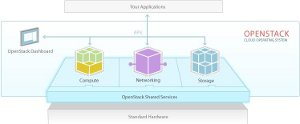
\includegraphics{images/openstack}}
\caption{Openstack at a glance.}
\label{fig:openstack}
\end{figure}


\section{Related Work}
Studies have been published to evaluate the applicability of the cloud for 
scientific computing. The works described below focus on the performance 
evaluation of clouds for scientific applications.

\cite{walker_benchmarking_2008} showed that a performance gap between running 
HPC applications on a baremetal cluster and on an Amazon's EC2 provisioned 
cluster. They suggested that in order for cloud computing to be a viable 
alternative for HPC, providers must improve in the area of network 
interconnection.

\cite{evangelinos_cloud_2008} found that Amazon's EC2 may be a credible 
solution for on-demand and small-sized HPC applications. They supported this 
conclusion by running a low-order coupled atmosphere-ocean simulation on EC2.

\cite{ekanayake_high_2010} presented performance analysis of HPC applications on virtualized 
resources. They concluded that cloud techonologies work well for pleasingly-
parallel problems. The main limitation of cloud technologies is the high 
overhead for applications with complex communication patterns, even with large 
data sets. 

\cite{jackson_performance_2010} compared the performance of conventional 
HPC platforms to Amazon EC2. Their results showed that EC2 is six times slower 
than a typical mid-range Linux cluster, and twenty times slower than a modern 
HPC system. This is mainly because of the communication overhead. They also 
noted that variability in performance can be significant due to the shared 
nature of the cloud environment.

\cite{zhai_cloud_2011} conducted a comprehensive comparison of the performance 
of a baremetal cluster(connected using Infiniband) and a cluster deployed 
using Amazon's Cluster Compute Instances (CCI). The study also revealed that
running MPI applications in the cloud yielded more positive results compared to 
published results. They also highlight the flexibility and elasticity advantage of 
using cloud.   

\cite{mauch_high_2013} presented the High Performance Cloud Computing (HPC2) 
model. This model enables the provisioning of elastic virtual clusters which 
avoids the initial cost for physically owned hardware. They also presented a 
novel architecture for HPC IaaS clouds which support InfiniBand with QoS 
mechanisms since existing platforms still use Ethernet.

\cite{exposito_performance_2013} concluded that HPC application scalability 
depends mainly on the communication performance. Their study involved the use 
of Amazon's EC2 Cluster Compute Instances (CCI) platform targeted to HPC 
applications. This platform provides access to a high-speed 
network(10 Gigabit Ethernet).

\cite{ludescher_cloud-based_2013} presented a novel code execution framework
(CEF) to execute problem solving environment (PSE) source code in parallel 
on a cloud. The paper emphasized that the use of a public cloud can result to 
a magnitude of cost savings.

A recurring observation based on the above works is that primarily, the public 
cloud suffers from variability in performance probably because of multitenancy 
and limited network infrastructure.

\section{Methodology}
P2C is a combination of hardware, software, and network configuration. 
In this section we describe how these are combined to achieve the desired 
results.

\subsection{Hardware}
P2C uses commercial-off-the-shelf(COTS) hardware. The cloud controller(1 unit) 
and compute nodes(2 units) are four-core Intel(R) Core(TM) i3-2000 3.10GHz CPU 
with 4GB RAM and 100GB disk. A 1GBps, 16-port Dell PowerConnect 2716 switch 
connects the controller and the nodes. Figure~\ref{fig:nodes} and 
Figure~\ref{fig:switch} show the nodes and the switch respectively.

\begin{figure}
\centerline{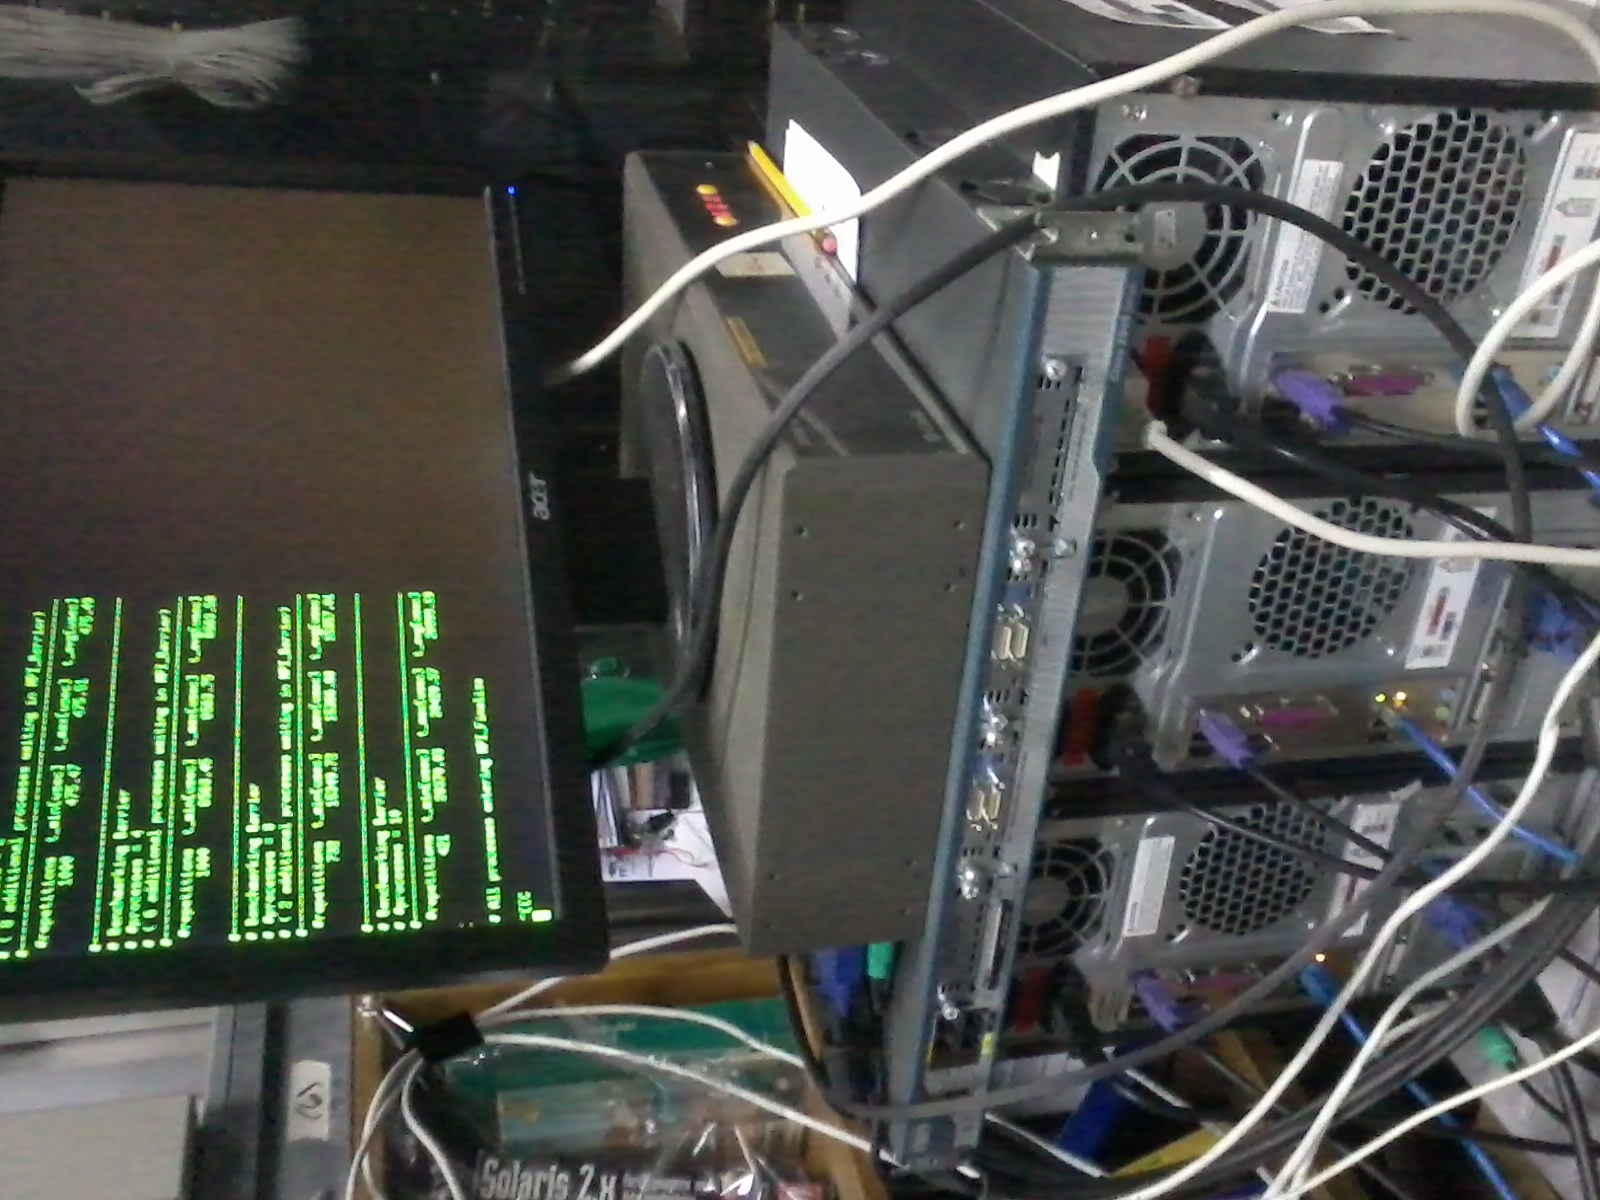
\includegraphics{images/nodes}}
\caption{Hardware used in P2C.}
\label{fig:nodes}
\end{figure}

\begin{figure}
\centerline{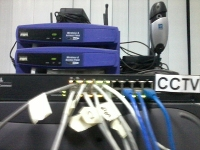
\includegraphics{images/switch}}
\caption{Switch used in P2C.}
\label{fig:switch}
\end{figure}


\subsection{Software}
P2C uses the Havana version of Openstack. Figure~\ref{fig:network} shows what 
Openstack component is installed on each node. The host openstack-clc is the 
cloud controller and contains Keystone, Glance, Nova, Horizon, and Nova-Network.
The compute nodes, hosts openstack-compute-01 and openstack-compute-02, has 
Nova and Nova-Network installed. Ubuntu Server 12.01 was used as the host 
operating system for the nodes. 

\subsection{Network Topology}
Figure~\ref{fig:network} shows the network topology of P2C. Each node has two 
NICs connected to different networks. The first NIC is connected through a 
100MBps Ethernet accesible through the institute's network (10.0.3.0/24 subnet).
This setup allows staff to access the instances from their own computers
through the bridge interface in the nodes. The second NIC is connected to a 
1GBps Ethernet(192.168.1.0/24 subnet) used for managing the setup. 

\begin{figure}
\centerline{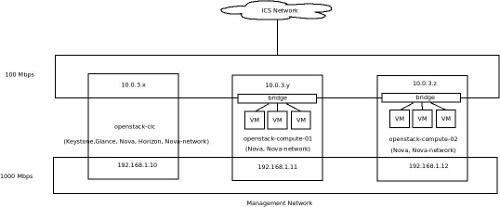
\includegraphics{images/network}}
\caption{Network topology}
\label{fig:network}
\end{figure}


\subsection{VM Images}



\subsection{vcluster}

\subsection{Benchmarks}


\section{Results and Discussion}

Figure~\ref{fig:p2c-dashboard} shows the P2C dashboard.


\begin{figure}
\centerline{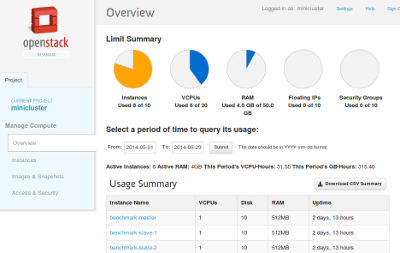
\includegraphics{images/p2c-dashboard}}
\caption{P2C Dashboard}
\label{fig:p2c-dashboard}
\end{figure}

\section{Conclusions}

% Acknowledgments
\begin{acks}
The author would like to thank the Lord.
\end{acks}

% Bibliography
\bibliographystyle{ACM-Reference-Format-Journals}
\bibliography{cloudcomp}
%\bibliography{acmsmall-sample-bibfile}
                             % Sample .bib file with references that match those in
                             % the 'Specifications Document (V1.5)' as well containing
                             % 'legacy' bibs and bibs with 'alternate codings'.
                             % Gerry Murray - March 2012

% History dates
\received{May 2014}{June 2014}{June 2014}

\end{document}
% End of v2-acmsmall-sample.tex (March 2012) - Gerry Murray, ACM


